\documentclass[BoSSSForSolvingConservationLaws.tex]{subfiles}
\begin{document}
Considering linear equation components, if time discretization is explicit still the nonlinear quadrature is applicable. It uses DG coordinates of domain fields known from the previous time step or the initial value but if the method is implicit, spatial discretization of the terms like following integrals for a scalar conservation law
\begin{align}
\label{VolumeIntegral-Implicit}
-\int_{K_j} [\vec{f}_j^{h,(n+1)}\cdot \nabla \phi_{jm} - q_j^{h,(n+1)} \phi_{jm}] d\vec{x},&\qquad 0\leq m \leq N_p-1\\
\label{EdgeIntegral-Implicit}
\int_{E_i} \hat{n}\cdot (\vec{f}_j^*)^{(n+1)} \phi_{jm} d\vec{x}, \qquad E_i \in \partial K_j,&\qquad 0\leq m \leq N_p-1
\end{align}
leads to a matrix formulation for the whole domain.
\begin{align*}
\textbf{W}^{(n+1)}&=A\textbf{U}^{(n+1)}+B\\
\label{LinearQuadrature-MatrixForm}
\begin{bmatrix}
\tilde{w}_{(0,0,0)}\\
\vdots\\
\tilde{w}_{(\gamma,j,m)}\\
\vdots\\
\end{bmatrix}_{Mrow}&=
\begin{bmatrix}
a_{(0,0,0),(0,0,0)} & \dots  & a_{(0,0,0),(f,j,n)} \dots \\
\vdots              & \ddots & \vdots\\
a_{(\gamma,j,m),(0,0,0)} &  \dots & a_{(\gamma,j,m),(f,j,n)} \dots\\
\vdots & \ddots & \vdots
\end{bmatrix}_{Mrow\times Ncol}
\begin{bmatrix}
\hat{u}_{(0,0,0)}\\
\vdots\\
\hat{u}_{(f,j,n)}\\
\vdots
\end{bmatrix}_{Ncol}+
\begin{bmatrix}
b_{(0,0,0)}\\
\vdots\\
b_{(\gamma,j,m)}\\
\vdots\\
\end{bmatrix}_{Mrow}
\end{align*}

Matrix $\vec{U}$ is the matrix of unknown DG coefficients of domain fields to be found. Index to this matrix comes from coordinate mapping (see section \ref{sec:CoordinateMapping}, \nameref{sec:CoordinateMapping}) of domain fields. Matrices $A$ and $B$ are found from spatial discretization of linear equation components. $A$ is called the \emph{matrix} and $B$ is called the \emph{affine offset} of the linear equation components. The affine offset usually results from the boundary conditions. Rows of matrix $A$ and affine offset $B$ correspond to coordinate mapping of codomain variables ($m\_RowMap$) and number of the them is $Mrow=J\times \sum_{\gamma=0}^{\Gamma-1} N_{p\gamma-max}$. Columns of matrix $A$ correspond to coordinate mapping of the domain variables ($m\_ColMap$). Number of columns is $Ncol=J\times\sum_{\lambda=0}^{\Lambda-1} N_{p\lambda-max}$. Matrix $\vec{W}$ is result of spatial discretization of equations (see section \ref{sec:SpatialDifferentialOperator}, \nameref{sec:SpatialDifferentialOperator}) and its index comes from coordinate mapping of codomain variables

\subsection*{Implementation in BoSSS}
Matrix $A$ (m\_matrix)\coderm{BoSSS.Foundation.Quadrature.Linear.LECQuadratureCommon.m\_Matrix} is an MsrMatrix (see section \ref{sec:MsrMatrix}, \nameref{sec:MsrMatrix}) and matrix $B$ \\($m\_AffineOffset$)\coderm{BoSSS.Foundation.Quadrature.Linear.LECQuadratureCommon.m\_AffineOffset} is a list of doubles. Indices to matrix $A$, $row$ and $col$  are global unique coordinate indices (see section \ref{sec:CoordinateMapping}, \nameref{sec:CoordinateMapping}) but index to the affine offset $B$ is a local index $rowloc$ found\coderm{BoSSS.Foundation.UnsetteledCoordinateMapping.Global2LocalIndex(...)} from the global index $row$ of matrix $A$, because the matrix $B$ is distributed over the processors.\\
Matrix $\vec{W}$ is result of evaluation of the spatial differential operator. Matrices $A$ and $B$ are created and computed by the evaluator of the spatial differential operator. If these matrices change with time they can be recomputed where ever they are required. There is an option to specify that only the affine offset $B$ needs to be computed. This would be the case for example when boundary conditions of the problem change with time.\\
Computing the matrices $A$ and $B$ is performed by defining and executing linear volume\coderm{BoSSS.Foundation.Quadrature.Linear.LECVolumeQuadrature} and edge\coderm{BoSSS.Foundation.Quadrature.Linear.LECQuadratureEdge} quadratures. Remembering from the general quadrature (see section \ref{sec:QuadRules}), each integral is referred to by an index used for accessing arrays of evaluation results of the integrands and the quadrature results. These indices in case of linear quadrature are provided by a map, $MyOwnMapping$\coderm{BoSSS.Foundation.Quadrature.Linear.LECQuadratureCommon.MyOwnMapping}. To distinguish between entries corresponding to matrix $A$ and affine offset $B$, indices are stored separately in this mapping. Index $m\_Mapping[\gamma,m,\delta,n]$\coderm{BoSSS.Foundation.Quadrature.Linear.LECQuadratureCommon.MyOwnMapping.m\_Mapping} refers to an integral corresponding to matrix $A$ and index $m\_MappingOffset[\gamma,m]$\coderm{BoSSS.Foundation.Quadrature.Linear.LECQuadratureCommon.MyOwnMapping.m\_MappingOffset} refers to an integral corresponding to affine offset $B$. $\gamma$ and $m$ are indices for codomain variables and test functions. $\delta$\nomenclature{$\delta$}{index for domain fields on which a codomain variable $\gamma$ depends} is index for domain fields on which the codomain variable $\gamma$ depends (not all domain fields). These fields are called \emph{dependent fields}\coderm{BoSSS.Foundation.Quadrature.Linear.LECQuadratureCommon.MyOwnMapping.m\_DependentfieldsNames}. $n$ is basis polynomial index for the dependent field $\delta$.

\subsection{Linear quadrature}
For creating a linear quadrature\coderm{BoSSS.Foundation.Quadrature.Linear.LECQuadratureCommon} we need to know, if only the affine offset $B$ is going to be computed (the boolean variable $OnlyAffine$), and also like nonlinear quadrature, the quadrature type ($Volume$, $Edge$), number of integrals and required order of precision for integration\coderm{BoSSS.Foundation.Quadrature.Linear.LECQuadratureCommon.FindQuadratureOder}. By creation of a linear quadrature\coderm{BoSSS.Foundation.Quadrature.Linear.LECQuadratureCommon.LECQuadratureCommon(...)} the mapping $MyOwnMapping$ is created and equation components of type linear flux\coderm{BoSSS.foundation.ILinearFlux} are sorted (like in the case of nonlinear quadrature) for each codomain variable (equation) $\gamma$. In the mapping, indices corresponding to the matrix $A$ which are stored in $m\_Mapping[\gamma,m,\delta,n]$ are created by making loops over codomain variables, test functions, dependent variables of codomain variables\coderm{BoSSS.Foundation.SpatialDifferentialOperator.CollectDependentVariables(...)} and their basis polynomials (with the outer loop over codomain variables). Indices are continued by making another loop over codomain variables and test functions and stored in $m\_MappingOffset[\gamma,m]$ for the affine offset $B$. If only affine offset is going to be computed then there is no index assigned for the matrix. Total number of integrals in this mapping, $m\_length$, is sum of number of integrals related to matrix $A$ and number of integrals $m\_LengthOffset$ related to affine offset $B$.
\begin{align*}
m\_Length&=\sum_{\gamma=0}^{\Gamma-1}\sum_{m=0}^{N_{p\gamma}-1}\sum_{\delta=0}^{\Delta(\gamma)-1}N_{p\delta}+\sum_{\gamma=0}^{\Gamma-1}N_{p\gamma}\\
m\_LengthOffset&=\sum_{\gamma=0}^{\Gamma-1}N_{p\gamma}
\end{align*}

\subsubsection{Linear volume quadrature}
\label{sec:LinearVolumeQuadrature}
When a volume quadrature\coderm{BoSSS.Foundation.Quadrature.Linear.LECVolumeQuadrature} is created\coderm{BoSSS.Foundation.Quadrature.Linear.LECVolumeQuadrature.LECVolumeQuadrature(...)} equation components of type linear source\coderm{BoSSS.Foundation.ILinearSource} are sorted for all codomain variables.\\
To show entries to matrix $A$ and affine offset $B$ computed by the volume quadrature, we consider the volume integral of the scalar conservation law, equation \eqref{VolumeIntegral-Implicit} and substitute the linear flux and linear source formulations (see section \ref{sec:FluxAndSource}, \nameref{sec:FluxAndSource}).
\[
-\int_{K_j} [(A_F u_j^h+B_F)\cdot \nabla \phi_{jm} - (A_S u_j^h+B_S) \phi_{jm}] d\vec{x},\qquad 0\leq m \leq N_p-1
\]
Flux matrix $A_F$ and flux affine offset $B_F$ have dimensions $D\times1$ and source matrix $A_S$ and source affine offset $B_S$ are double values for this example. Substituting the domain field $u_j^h$
\[
-\int_{K_j} [\bigg( A_F \sum_{n=0}^{N_p-1} \hat u_{jn} \phi_{jn}+B_F \bigg)\cdot \nabla \phi_{jm}-\bigg( A_S \sum_{n=0}^{N_p-1} \hat u_{jn} \phi_{jn}+B_S \bigg)\phi_{jm}] d\vec{x},\qquad 0\leq m \leq N_p-1
\]
For simplicity considering only the part related to the flux, for $0\leq m \leq N_p-1$
\begin{align*}
-\int_{K_j}
\bigg(\begin{bmatrix}
(\nabla \phi_{jm}\cdot A_F) \phi_{j0} & \dots & (\nabla \phi_{jm}\cdot A_F) \phi_{jn}  & \dots
\end{bmatrix}_{N_P}
&\begin{bmatrix}
\hat u_{j0}\\
\vdots\\
\hat u_{jn}\\
\vdots
\end{bmatrix}_{N_P}+\nabla \phi_{jm}\cdot B_F \bigg)
d\vec{x}\\
\begin{bmatrix}
-\int_{K_j} (\nabla \phi_{jm}\cdot A_F) \phi_{j0} d\vec{x} & \dots & -\int_{K_j} (\nabla \phi_{jm}\cdot A_F) \phi_{jn} d\vec{x}  & \dots
\end{bmatrix}_{N_P}
&\begin{bmatrix}
\hat u_{j0}\\
\vdots\\
\hat u_{jn}\\
\vdots
\end{bmatrix}_{N_P}-\int_{K_j} \nabla \phi_{jm}\cdot B_F d\vec{x}
\end{align*}
We arrive at the following matrix form
\[
\begin{bmatrix}
-\int_{K_j} (\nabla \phi_{j0}\cdot A_F) \phi_{j0} d\vec{x} & \dots & -\int_{K_j} (\nabla \phi_{j0}\cdot A_F) \phi_{jn} d\vec{x}  \dots\\
\vdots                                                     &\ddots &\vdots\\
-\int_{K_j} (\nabla \phi_{jm}\cdot A_F) \phi_{j0} d\vec{x} & \dots & -\int_{K_j} (\nabla \phi_{jm}\cdot A_F) \phi_{jn}
d\vec{x}  \dots\\
\vdots                                                     &\ddots &\vdots\\
\end{bmatrix}_{N_P \times N_P}
\begin{bmatrix}
\hat u_{j0}\\
\vdots\\
\hat u_{jn}\\
\vdots
\end{bmatrix}_{N_P}+
\begin{bmatrix}
-\int_{K_j} \nabla \phi_{j0}\cdot B_F d\vec{x}\\
\vdots\\
-\int_{K_j} \nabla \phi_{jm}\cdot B_F d\vec{x}\\
\vdots
\end{bmatrix}_{N_P}
\]
For this example of the scalar conservation law there are only one codomain and one domain variables but in general for each codomain variable $\gamma$ which depends on $\Delta$ domain variables, there are matrices $A_{F\gamma}$ with dimension $D\times \Delta$ and $A_{S\gamma}$ with dimension $\Delta$. Also there are affine offsets $B_{F\gamma}$ with dimension $D\times1$ and $B_{S\gamma}$ which are double values.\\
Comparing to this example, each component $a_{(\gamma,j,m),(f,j,n)}$ of matrix $A$ contains a term \\$-\int_{K_j}[ \sum_{d=0}^{D-1} \nabla \phi_{jm}(d) A_{F\gamma}(d,\delta) \phi_{jn}-\phi_{jm}A_{S\gamma}(\delta)\phi_{jn}] d\vec{x}$. $f$\coderm{BoSSS.Foundation.Quadrature.Linear.LECQuadratureCommon.MyOwnMapping.m\_DependentFieldsIndex}\nomenclature{$f$}{Index for fields of domain variables} is index of the dependent field $\delta$ in list of domain variables. Each component $b_{(\gamma,j,m)}$ of the affine offset $B$  has a term \\$-\int_{K_j} [\sum_{d=0}^{D-1}\nabla \phi_{jm}(d) B_{F\gamma}(d)-\phi_{jm}B_{S\gamma}] d\vec{x}$ computed by the volume quadrature. Number\coderm{BoSSS.Foundation.Quadrature.Linear.LECQuadratureCommon.MyOwnMapping.m\_Length} of integrals for a volume quadrature is equal to number of integrals in $MyOwnMapping$.
\[
N_{integral}=m\_Length
\]
Followings are quadrature details specific to linear volume quadrature.
\begin{itemize}
\item \textbf{Creating node set family}\\
The same as for the nonlinear quadrature the node set family has only one set of nodes which are quadrature points of the quadrature rule.
\item \textbf{Specifying memory}\\
Besides the memory required for general quadrature, memory is allocated\coderm{BoSSS.Foundation.Quadrature.Linear.LECVolumeQuadrature.AllocateBuffers(...)} for parameter values.
\item \textbf{Finding values of test functions, gradient of test functions and basis polynomials}\\
Values of test functions, gradient of test functions and basis polynomials are found\coderm{BoSSS.Foundation.Quadrature.Linear.LECVolumeQuadrature.PostLockNodes(...)} and stored at $m\_TestFunctions[\gamma]$, $m\_GradientTestFunctions[\gamma]$ and $m\_BasisFunctions[\gamma][\delta]$.
\item \textbf{Evaluation of integrands}\\
Integrands in case of linear volume quadrature are $\sum_{d=0}^{D-1} \nabla \phi_{jm}(d) A_{F\gamma}(d,\delta) \phi_{jn}-\phi_{jm}A_{S\gamma}(\delta)\phi_{jn}$ for the matrix and $\sum_{d=0}^{D-1}\nabla \phi_{jm}(d) B_{F\gamma}(d)-\phi_{jm}B_{S\gamma}$ for the affine offset. In the following procedure for evaluation of the integrands, steps \ref{StartOfLoopVolume} to \ref{EndOfLoopVolume} are performed inside loops over cells $j$, nodes $n\_node$ of the node set and codomain variables $\gamma$.
\begin{enumerate}
\item \textbf{Evaluation of parameter variables}\\
Fields in parameter variables coordinate mapping are evaluated at the node set and stored at $m\_ParamFieldValues[p][j,n\_node]$. $p$ is index for parameter variables.
\item \textbf{Transform nodes to global coordinates}\\
As in the case of nonlinear volume quadrature $m\_NodesGlobalCoords[j,n\_node,d]$ stores the global coordinates of the nodes in the node set.
\item \textbf{Sum up flux matrices and affine offsets}\\
\label{StartOfLoopVolume}
Flux matrices $FluxesComponents[\gamma][c][d,\delta]$ and affine offsets $FlxCompOffset[d]$ are first found\coderm{BoSSS.Foundation.Quadrature.Linear.LECVolumeQuadrature.SumUpFluxes(...)} from linear fluxes\coderm{BoSSS.Solution.Utils.LinearFlux.Flux(...)} of equation components of each codomain variable $\gamma$. $c$\nomenclature{$c$}{Index for equation components} is index for equation components. Then they are added up over all equation components to provide the flux matrices $FlxTotTransf[d,\delta]$ and affine offset $FlxTotOffsetTransf[d]$. The flux matrices and the affine offset are multiplied by the inverse transformation matrix $((M_j)^{-1})^T$ of cell $j$ and scaled by $\frac{1}{|det(M_j)|}$ for the matrices and $\frac{1}{\sqrt{|det(M_j)|}}$ for the offset to account for transformation of the term $\vec{f}_j^h\cdot \nabla \phi_{jm}$ in to physical domain.
\item \textbf{Sum up source matrices and affine offsets}\\
Source matrix $SourceComponents[\gamma][c][\delta]$ and affine offsets are found\coderm{BoSSS.Foundation.Quadrature.Linear.LECVolumeQuadrature.SumUpSources(...)} from linear sources\coderm{BoSSS.Solution.Utils.LinearSource.Source(...)} of equation components of each codomain variable $\gamma$ and then added up over all equation components to provide the source matrix $SrcTot[\delta]$ and affine offset $SrcTotalOffset$, which is a double value. The matrix and the affine offset of the source are scaled with the same scale factors as for the flux.
\item \textbf{Multiplying flux matrix and affine offset by gradient of test functions}\\
The flux matrix and the affine offset of codomain variable $\gamma$ and dependent variable $\delta$ are multiplied by the gradient of test function $m$ and accumulated.
\begin{align*}
s+&=FlxTotTransf[d,\delta] \times m\_GradientTestFunctions[\gamma][n\_node, m, d]\\
ss+&=FlxTotOffsetTransf[d] \times m\_GradientTestFunctions[\gamma][n\_node, m, d]
\end{align*}
\item \textbf{Multiplying source matrix and affine offset by test functions}\\
The source matrix and the affine offset of codomain variable $\gamma$ and dependent variable $\delta$ are multiplied by the test function $m$ and subtracted from the corresponding sums of the flux matrix and offset. $ss$ is summation of integrands that correspond to affine offset $B$ of the linear quadrature.
\begin{align*}
s-&=SrcTot[\delta] \times m\_TestFunctions[\gamma][n\_node, m]\\
ss-&=SrcTotalOffset \times m\_TestFunctions[\gamma][n\_node, m]
\end{align*}
\[
EvalResult[j, n\_node, m\_MyOwnMapping.m\_MappingOffset[\gamma, m]] = ss
\]
\item \textbf{Multiplying flux and source matrices with basis polynomials}\\
\label{EndOfLoopVolume}
The computed sum $s$ is multiplied by the basis polynomial $n$. $sum$ is summation of integrands that correspond to matrix $A$ of the linear quadrature.
\begin{align*}
&sum=s \times m\_BasisFunctions[\gamma][\delta][n\_node,n]\\
&EvalResult[j, n\_node, m\_MyOwnMapping.m\_Mapping[\gamma, m, \delta, n]]=sum
\end{align*}
\end{enumerate}
\item \textbf{Saving integration results}\\
Results of integration are subtracted from the output of the spatial differential operator by making a loop over all cells $j$.
\begin{align*}
m\_Matrix[row,col]& -=\\
&ResultsOfIntegration[j,m\_MyOwnMapping.m\_Mapping[\gamma,m,\delta,n]]
\end{align*}
\begin{align*}
m\_AffineOffset&[rowLoc] -=\\
&ResultsOfIntegration[j, m\_MyOwnMapping.m\_MappingOffset[\gamma, m]]
\end{align*}
As mentioned before index $row$ is found from indices $(\gamma,j,m)$ and index $col$ from $(f,j,n)$ by coordinate mapping of codomain and domain variables and $f$ is index of the dependent field $\delta$ in list of domain variables. Index $rowLoc$ is local row index found from $row$.
\end{itemize}

\newpage
\subsubsection{Linear edge quadrature}
\label{sec:LinearEdgeQuadrature}
To show entries to matrix $A$ and affine offset $B$ computed by linear edge quadrature, we consider the edge integral of the scalar conservation law, equation \eqref{EdgeIntegral-Implicit} and substitute the linear flux for an inner edge (see section \ref{sec:FluxAndSource} and \nameref{sec:FluxAndSource}) as an example.
\[
\int_{E_i} (A_I u_j^h+A'_I u_{j'}^h+B_I) \phi_{jm} d\vec{x}, \qquad E_i \in \partial K_j,\qquad 0\leq m \leq N_p-1
\]
$A_I$ and $A'_I$ are inner edge matrices related to the first neighbor, cell $j$ and second neighbor cell $j'$. $B_I$ is inner edge affine offset. Substituting the domain field polynomial representations in both neighbors
\begin{align*}
&\int_{E_i} (A_I \sum_{n=0}^{N_p-1} \hat u_{jn} \phi_{jn}+A'_I \sum_{n=0}^{N_p-1} \hat u_{j'n} \phi_{j'n}+B_I) \phi_{jm} d\vec{x}=\\
&\sum_{n=0}^{N_p-1} (\int_{E_i} \phi_{jm} A_I  \phi_{jn} d\vec{x}) \hat u_{jn}+
\sum_{n=0}^{N_p-1} (\int_{E_i} \phi_{jm} A'_I  \phi_{j'n} d\vec{x}) \hat u_{j'n}+
\int_{E_i} \phi_{jm} B_I d\vec{x}
\end{align*}
The first two integrals correspond to matrix $A$ and the third one to matrix $B$. These integrals which have test function $\phi_{jm}$ are computed in cell $j$ the first neighbor of edge $i$. In general case, for each codomain variable $\gamma$ which depends on $\Delta$ domain variables, there are matrices $A_{I\gamma}$ and $A'_{I\gamma}$ with dimension $\Delta$ and affine offset $B_{I\gamma}$ which is a double value. The term $\int_{E_i} \phi_{jm} A_{I\gamma}(\delta) \phi_{jn} d\vec{x}$ is accumulated at entry $a_{(\gamma,j,m),(f,j,n)}$, the term $\int_{E_i} \phi_{jm} A'_{I\gamma}(\delta) \phi_{j'n} d\vec{x}$ at $a_{(\gamma,j,m),(f,j',n)}$ and the term $\int_{E_i} \phi_{jm} B_{I\gamma} d\vec{x}$ at $b_{(\gamma,j,m)}$.\\
Now if we consider the same edge $i$ but the integral to be calculated for the second neighbor cell $j'$, we have the following integral
\[
-\int_{E_i} (A_I u_j^h+A'_I u_{j'}^h+B_I) \phi_{j'm} d\vec{x}, \qquad E_i \in \partial K_{j'},\qquad 0\leq m \leq N_p-1
\]
The minus sign must be considered for the flux in the second neighbor because the normal vector to the edge is considered to point from the first neighbor (specified by \emph{In}) to the second neighbor (specified by \emph{Out}). With the same procedure as the above we arrive at the following terms for cell $j'$. The term $\int_{E_i} \phi_{j'm} A_{I\gamma}(\delta) \phi_{jn} d\vec{x}$ contributes to $a_{(\gamma,j',m),(f,j,n)}$. The term $\int_{E_i} \phi_{j'm} A'_{I\gamma}(\delta) \phi_{j'n} d\vec{x}$ contributes to $a_{(\gamma,j',m),(f,j',n)}$ and the affine offset term $\int_{E_i} \phi_{j'm} B_{I\gamma} d\vec{x}$ contributes to $b_{(\gamma,j',m)}$.\\
In arrays for evaluation results of the integrands and quadrature results, first the integrals related to the first neighbor are stored and then integrals related to the second neighbor. As shown in figure \ref{fig:MOM} at each part related to integrals of the neighbors, first integrals corresponding to matrix $A$ with basis polynomials of the first neighbor, then integrals corresponding to matrix $A$ with basis polynomials of the second neighbor and after them integrals corresponding to the affine offset $B$ are stored. These parts are accessed by indices shown in the figure; for example $m\_iOut\_In$ specifies the starting point of the integrals related to the second neighbor.
\begin{figure}[h]
\begin{center}
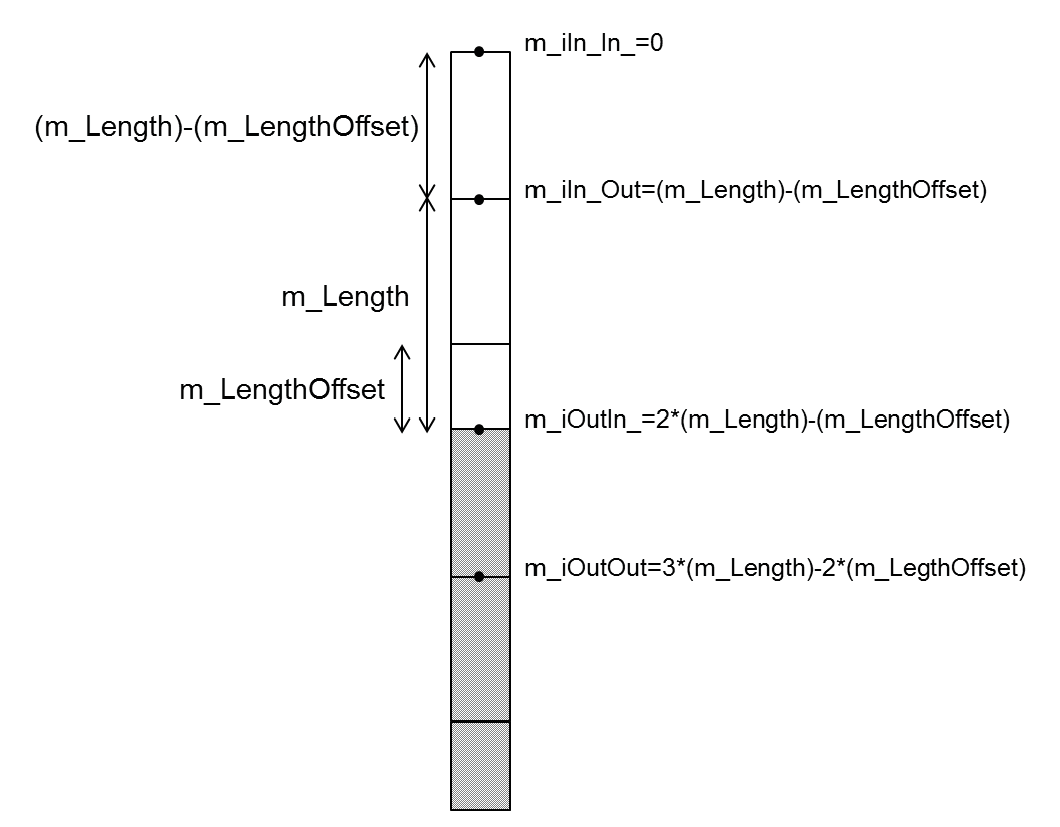
\includegraphics[width=12cm]{figures/MOM}
\end{center}
\label{fig:MOM}
\caption{Mapping used for linear quadrature. \emph}
\end{figure}
Number of integrals calculated for each edge $i$ in linear edge quadrature is $N_{integral}= 4\times m\_Length- 2\times m\_LengthOffset$.

\begin{itemize}
\item \textbf{Creating node set family}\\
creating the node set family is the same as for the nonlinear edge quadrature.
\item \textbf{Specifying memory}\\
Besides the memory required for general quadrature, memory is allocated\coderm{BoSSS.Foundation.Quadrature.Linear.LECQuadratureEdge.AllocateBuffers(...)} for parameter values in both neighbors.
\item \textbf{Finding values of test functions and basis polynomials}\\
Values of test functions and basis polynomials are found\coderm{BoSSS.Foundation.Quadrature.Linear.LECQuadratureEdge.PostLockNodes(...)} at the node set family. They are stored at $m\_TestFunctions\_1stCell[e, \gamma][n\_node,m]$ and \\$m\_BasisFunctions\_1stCell[e, \gamma][\delta][n\_node,n]$ corresponding to the first neighbors and at $m\_TestFunctions\_2ndCell[e, \gamma, k][n\_node,m]$ and \\$m\_BasisFunctions\_2ndCell[e, \gamma, k][\delta][n\_node,n]$ corresponding to the second neighbors if it exists. $e$ is index for edges in volume simplex and $k$ is index for inter cell transformations.
\item \textbf{Evaluation of integrands}\\
Integrands to be evaluated are $\phi_{jm} A_{I\gamma}(\delta) \phi_{jn}$, $\phi_{jm} A'_{I\gamma}(\delta) \phi_{j'n}$ and $\phi_{jm} B_{I\gamma}$ for the first neighbor and $\phi_{j'm} A_{I\gamma}(\delta) \phi_{jn}$, $\phi_{j'm} A'_{I\gamma}(\delta) \phi_{j'n}$ and $\phi_{j'm} B_{I\gamma}$ for the second neighbor if it exists. For a boundary edge there is no second neighbor so there are only $\phi_{jm} A_{B\gamma}(\delta) \phi_{jn}$ and $\phi_{jm} B_{B\gamma}$ to be computed. In the following procedure of evaluation of integrands, steps \ref{StartOfLoopEdge} to \ref{EndOfLoopEdge} are performed inside loops over edges $i$, nodes of the node set family $n\_node$ and codomain variables $\gamma$.
\begin{enumerate}
\item \textbf{Evaluation of parameter variables}\\
The Fields in parameter variables coordinate mapping are evaluated at the node set family and stored for the first and second neighbors at \\$m\_ParameterValuesEdge1[p][j,n\_node]$ and $m\_ParameterValuesEdge2[p][j',n\_node]$.
\item \textbf{Transform nodes to global coordinates}\\
As in the case of nonlinear edge quadrature, global coordinates of the nodes are found and stored at $m\_NodesGlobalCoords[i,n\_node,d]$.
\item \textbf{Sum up flux matrices and affine offsets}\\
\label{StartOfLoopEdge}
Flux matrices $FluxesComponentsIn[\gamma][c][\delta]$ and $FluxesComponentsOut[\gamma][c][\delta]$ and affine offsets are found\coderm{BoSSS.Foundation.Quadrature.Linear.LECQuadratureEdge.EvalFluxes(...)} from linear inner edge\coderm{BoSSS.Solution.Utils.LinearFlux.InnerEdgeFlux(...)} and border edge\coderm{BoSSS.Solution.Utils.LinearFlux.BorderEdgeFlux(...)} fluxes and are added up over all equation components to provide the flux matrices $FluxesTotalIn[\delta]$ and $FluxesTotalOut[\delta]$ and affine offset $FlxTotalOffset$. The flux matrices are scaled by scale factors of cells $j$ and $j'$, $scale0=\frac{1}{\sqrt{|det(M_j)|}}$ and $scale1=\frac{1}{\sqrt{|det(M_j')|}}$.
\item \textbf{Multiplying flux matrices with basis polynomials and test functions}\\
Flux matrices for both neighbors are multiplied by the basis polynomials,
\begin{align*}
sIn &= FluxesTotalIn[\delta] \times m\_BasisFunctions\_1stCell[e, \gamma][\delta][n\_node,n]\\
sOut &= FluxesTotalOut[\delta] \times m\_BasisFunctions\_2ndCell[e, \gamma, k][\delta][n\_node,n]
\end{align*}
then multiplied by test functions of the first neighbor, scaled and stored as the integrand related to matrix $A$.
\begin{align*}
EvalResult&[i, n\_node, m\_iIn\_In\_ + m\_MyOwnMapping.m\_Mapping[\gamma, m, \delta, n]] =\\ &sIn\times scale0 \times m\_TestFunctions\_1stCell[e, \gamma][n\_node,m]\\
EvalResult&[i, n\_node, m_iIn\_Out + m\_MyOwnMapping.m\_Mapping[\gamma, m, \delta, n]] =\\ &sOut \times scale0 \times m\_TestFunctions\_1stCell[e, \gamma][n\_node,m]
\end{align*}
For the second neighbor the integrands are calculated and stored at
\begin{align*}
EvalResult&[i, n\_node, m\_iOutIn\_ + m\_MyOwnMapping.m\_Mapping[\gamma, m, \delta, n]] =\\ &sIn \times scale1 \times m\_TestFunctions\_2ndCell[e, \gamma, k][n\_node,m]\\
EvalResult&[i, n\_node, m\_iOutOut + m\_MyOwnMapping.m\_Mapping[\gamma, m, \delta, n]] =\\ &sOut \times scale1 \times m\_TestFunctions\_2ndCell[e, \gamma, k][n\_node,m]
\end{align*}
\item \textbf{Multiplying the affine offset by test functions}\\
\label{EndOfLoopEdge}
For the first and second neighbors
\begin{align*}
EvalResult&[i, n\_node, m\_iIn\_Out + m\_MyOwnMapping.m\_MappingOffset[\gamma, m]] =\\ &FlxTotalOffset \times m\_TestFunctions\_1stCell[e, \gamma][n\_node,m] \times scale0\\
EvalResult&[i, n\_node, m\_iOutOut + m\_MyOwnMapping.m\_MappingOffset[\gamma, m]] =\\ &FlxTotalOffset \times m\_TestFunctions\_2ndCell[e, \gamma, k][n\_node,m] \times scale1
\end{align*}
\end{enumerate}
\item \textbf{Saving integration results}\\
For the first neighbor results of the integration are added to matrix entries at the row $rowIn$ and columns $ColIn$ and $ColOut$. $rowIn$ is found from the coordinate mapping of the rows with indices $(\gamma, j, m)$. $ColIn$ is found from coordinate mapping of the columns from indices $(f,j,n)$ and $ColOut$ from $(f,j',n)$.
\begin{align*}
m\_&Matrix[rowIn, colIn] +=\\ &ResultsOfIntegration[i, m\_iIn\_In\_ + m\_MyOwnMapping.m\_Mapping[\gamma, m, \delta, n]]\\
m\_&Matrix[rowIn, colOut] +=\\ &ResultsOfIntegration[i, m\_iIn\_Out + m\_MyOwnMapping.m\_Mapping[\gamma, m, \delta, n]]\\
\end{align*}
For the second neighbor results of integration are subtracted from matrix entries at the row $rowOut$ and columns $ColIn$ and $ColOut$. $rowOut$ is found from the coordinate mapping of the rows with indices $(\gamma, j', m)$.
\begin{align*}
m\_&Matrix[rowOut, colIn] -=\\ &ResultsOfIntegration[i, m\_iOutIn\_ + m\_MyOwnMapping.m\_Mapping[\gamma, m, \delta, n]]\\
m\_&Matrix[rowOut, colOut] -=\\ &ResultsOfIntegration[i, m\_iOutOut + m\_MyOwnMapping.m\_Mapping[\gamma, m, \delta, n]]\\
\end{align*}
For the affine offset matrix, results of integration from the first neighbor are added at row $rowInLoc$ and for the second one subtracted at $rowOutLoc$. The local indices are found from the global indices $rowIn$ and $rowOut$.
\begin{align*}
m\_&AffineOffset[rowInLoc] +=\\ &ResultsOfIntegration[i, m\_iIn\_Out + m\_MyOwnMapping.m\_MappingOffset[\gamma, m]]\\
m\_&AffineOffset[rowOutLoc] -=\\ &ResultsOfIntegration[i, m\_iOutOut + m\_MyOwnMapping.m\_MappingOffset[\gamma, m]]\\
\end{align*}
\end{itemize}

\end{document} 